\documentclass[final]{beamer}
\usepackage[orientation=portrait,size=a0,scale=1.4]{beamerposter}
\usepackage[icelandic]{babel}
\usepackage[T1]{fontenc}
\usepackage{ragged2e}
\usepackage{lmodern}
\usepackage{fontspec}

\usepackage{tcolorbox}
\usepackage[rounded]{syntax}
\usepackage{hyperref} 

\hypersetup{pdfencoding=auto}
\setmainfont{Arial} 
\usetheme{vonmaster}
\graphicspath{{./figs/}{../report/figs/}}

% Syntax diagrams
\newenvironment{repnull}[0]{%
\begin{stack}
\\
\begin{rep}
}{%
\end{rep}
\end{stack}
}
\newenvironment{syntaxenv}[1]{%
\par\noindent\begin{minipage}{0.7\linewidth}\vspace{0.5em}\begin{quote}\noindent%
\hspace*{-2em}\synt{#1}:\hfill\par%
\noindent%
\begin{minipage}{\linewidth}\begin{syntdiag}%
}{%
\end{syntdiag}\end{minipage}\end{quote}\end{minipage}%
}

%\beamertemplategridbackground[1cm]% Display a grid to help align images

\title{Nútímaleg vefkennsla í notkun gagnasafna með opnum hugbúnaði} 
\author{Eiríkur Ernir Þorsteinsson} 
\institute{Iðnaðarverkfræði-, vélaverkfræði- og tölvunarfræðideild} 
\newcommand{\insertinstructor}{Hjálmtýr Hafsteinsson}  % Not official, but provided for consistency
\date{Maí 2017}

\begin{document}
\begin{frame}
\begin{tcolorbox}[standard jigsaw, height=97cm, colframe=orange, opacityback=0, sharp corners=all]
\begin{columns}[t]

\begin{column}{.47\linewidth}

\begin{block}{Yfirlit}
    Nútímalegur, gagnvirkur kennsluvefur fyrir skipulega byrjendakennslu í notkun gagnasafna er gerður. Meðal krafa sem gerðar voru til vefsins eru að hann skuli\ldots
    \begin{itemize}
        \item styðja íslensku
        \item leyfa nemendastýrða, ólínulega framvindu í gegnum efnisatriði
        \item bjóða upp á verklegar æfingar samþættar við lesefni
        % \item tryggja eignarrétt yfir gögnum sem safnast við notkun 
    \end{itemize}
    En kerfi sem uppfyllir allar þessar kröfur samtímis var ekki til.
\end{block}

\begin{block}{Áhersluatriði}

    \begin{subblock}{Vefurinn sem bók, ólínuleg framvinda} 
        Rafrænar kennslubækur hafa lengi verið til. Uppbygging hinnar hefðbundnu rafrænu kennslubókar hafa hins vegar sterkar rætur í uppbyggingu pappírsbóka, þar sem efnisatriði eru sett fram í fastri röð.

        Vefur hefur fleiri möguleika. Sú leið sem valin var er að setja textaefni fram sem safn greina. 
        Greinarnar geta tengst innbyrðis. Þessi tengsl eru nýtt til að veita nemanda ráðgjöf um næsta efnisatriði til að skoða, frekar en að láta niðurröðun efnisins á blaðsíður ráða ferðinni.
        \begin{figure}
            \caption{Dæmi um venslaðar greinar}
            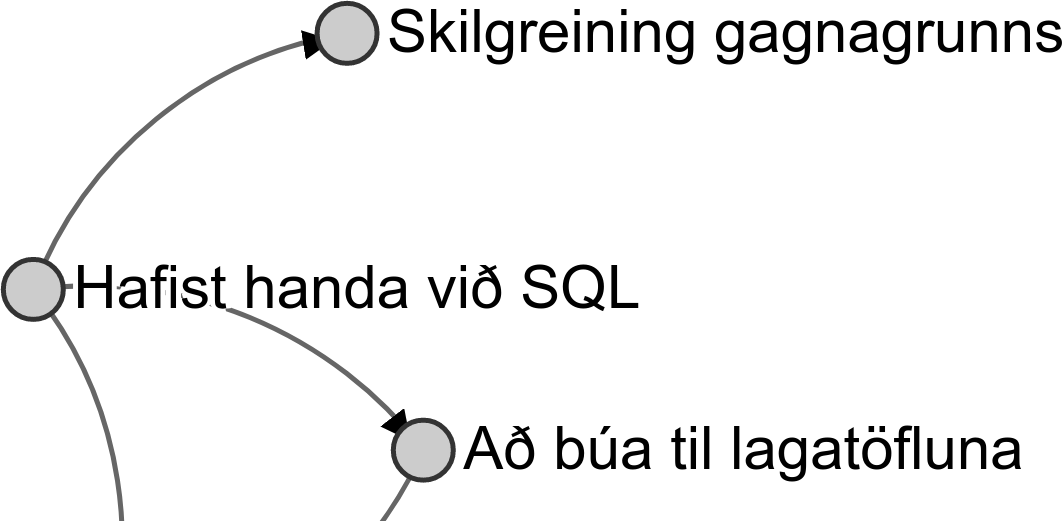
\includegraphics[width=0.5\textwidth]{relational-sections}
        \end{figure}
    \end{subblock}

    \begin{subblock}{Samþætting texta og æfinga}
        Algengt er að vefkennslukerfi séu fyrst og fremst æfingakerfi sem gera ráð fyrir að ítarlegri texta megi áfram finna í hefðbundnari kennslubók.

        Kennsluvefurinn styður samtengingu lesefnis og verklegra æfinga. Hægt er að tengja hverja grein lesefnis við æfingu eða æfingar. Tengingarnar eru notaðar nemendunum til ráðgjafar um hvaða æfingar megi kljást við næst.
    \end{subblock}

    \begin{subblock}{Opinn kóði, opið kennsluefni, ómiðstýrð dreifing}
        Fjölmörg kennslukerfi til kennslu í notkun gagnasafna hafa verið skrifuð innan háskólastofnana síðustu tvo áratugi. Oftast er um að ræða kerfi skrifuð af einstaklingum eða fámennum hópum til nota innan viðkomandi skólastofnunar. Kerfin hljóta notkun og af þeim hlýst fræðileg umfjöllun, en erfitt er að nálgast viðkomandi forrit og kennslugögn eftir að upphaflegir höfundar hverfa frá.
        
        Til að bjarga kennsluvefnum frá sömu örlögum er leitað í hugmyndasmiðju opins hugbúnaðar. Allur grunnkóði vefsins og allt textaefni hans eru gefin út undir opnu leyfi. Sömuleiðis er allur hugbúnaður frá 3. aðila sem vefurinn er háður líka opinn.
        \begin{figure}
            \caption{Allt textaefni vefsins er aðgengilegt undir Creative Commons leyfi.}
            
\includegraphics[width=0.3\linewidth]{cc-by-nc-sa}
        \end{figure}

        Þó opnun vefsins tryggi ekki langlífi hans ein og sér, þá er með þessum hætti gert líklegt að áhugasamir meistaranemar framtíðarinnar komi ekki að lokuðum dyrum.

        Opið eðli vefsins er líka hornsteinn í notkunarmódeli hans, sem gerir ráð fyrir að kennarar eða skólastofnanir setji upp sín eigin tilvik af vefnum út frá grunnkóðanum.
    \end{subblock}

\end{block}

\end{column}

\begin{column}{.47\linewidth}

\begin{block}{Útfærsla}
    Vefurinn er skrifaður í Python með notkun vefburðargrindarinnar Django. Nokkur atriði ber að nefna sérstaklega.

    \begin{subblock}{Sérhæfðar Markdown-viðbætur}
        Efnisinnsetning á kennsluvefnum er á Markdown-sniði.
        
        Markdown er einfalt ívafsmál, hannað til að auðvelda skrif. 
        En vegna einfeldninnar getur málið ekki uppfyllt allar kröfur sem gerðar voru til textaframsetningar. Fjórar viðbætur við Markdown-túlk voru skrifaðar fyrir kennsluvefinn, þeirra mikilvægastar eru viðbót til að leyfa framsetningu texta í tveimur dálkum og viðbót til að auðvelda innri tengingu greina.

        \begin{figure}
            \caption{Mállýsingar tveggja Markdown-viðbóta sem skrifaðar voru fyrir kennsluvefinn}
            \label{fig:markdown-internal-link}
            \begin{syntaxenv}{markdown-internal-link}
                `[' `[' <identifier>
                \begin{stack}
                    `|' <label>\\
                \end{stack}
                `]' `]'
            \end{syntaxenv}
            \begin{syntaxenv}{markdown-footnote}
                `[' `\textasciicircum' <note-identifier> `]' `[' <contents> `]'
            \end{syntaxenv}
        \end{figure}
    \end{subblock}

    \begin{subblock}{Markviss textaframsetning}
        Þar sem kennsluvefurinn skal gegna hlutverki kennslubókar er textaframsetning lykilatriði.
        
        Hönnun vefsins einkennist af notkun css-safnsins Tufte CSS, sem er hannað út frá hugmyndum fræðimannsins Edward Tufte um framsetningu texta. Meðal áberandi stílbragða er mikil notkun spássíugreina og samþjöppun texta og mynda.
    \end{subblock}

    \begin{subblock}{Greining nemendafyrirspurna}
        Greining á SQL-fyrirspurnum er umfangsmikið vandamál sem hlotið hefur töluverða athygli í rannsóknum.

        Aðalaðferð kennsluvefsins við að greina fyrirspurnir er samanburður á niðurstöðumengjum, sem framkvæmdur er í skammlífum, einangruðum gagnagrunnstilvikum.

        \begin{figure}
            \caption{Keyrsla nemendafyrirspurnar}
            \begin{center}
            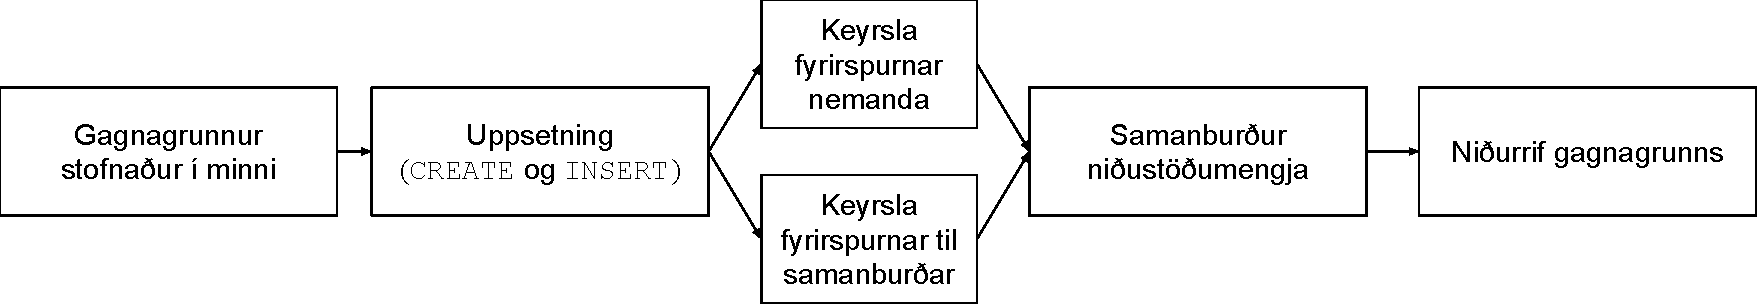
\includegraphics[width=\linewidth]{keyrsla-fyrirspurnar-larett}
        \end{center}
        \end{figure}

        Þegar ekki er mögulegt að beita mengjasamanburðaraðferðinni er einfaldur textasamanburður notaður til að veita nemendum endurgjöf.
    \end{subblock}
\end{block}

\begin{block}{Að nálgast hugbúnaðinn}
    Vefurinn er tilbúinn til tilraunanotkunar í kennslustofu.

    Hægt er að nálgast allan grunnkóða vefsins á Github-síðu höfundar. Þar má einnig finna uppsetningarleiðbeiningar til hýsingar á eigin vefþjóni.

    \url{https://github.com/Ernir/sql-web}
    
    \begin{center}
        \begin{figure}
            \caption{QR-kóði. Skannið til að nálgast grunnkóða vefsins.}
            
\includegraphics[width=0.25\linewidth]{qr-code}
        \end{figure}
    \end{center}
\end{block}

\end{column}

\end{columns}
\end{tcolorbox}
\end{frame}

\end{document}